
\documentclass[letterpaper, 10 pt, conference]{article}  % Comment this line out if you need a4paper

\usepackage{aaai}


\usepackage{times}
\usepackage[utf8]{inputenc}
\usepackage[small]{caption}
\usepackage{subcaption}
\usepackage{comment}
\usepackage{multirow}			

%\usepackage{gensymb}
%\usepackage{array}
%\usepackage{hyperref}
%\usepackage{tikz-er2}

\usepackage{amsfonts}
\usepackage{amsmath} % assumes amsmath package installed
\usepackage{amssymb}  % assumes amsmath package installed
\usepackage{euler}
%\usepackage{newtxtext, newtxmath}

\usepackage{graphicx}
\usepackage{graphics} % for pdf, bitmapped graphics files
%\usepackage{mathptmx} % assumes new font selection scheme installed
\usepackage{url}
\usepackage{rotating}
\usepackage[usenames, dvipsnames]{color}
\usepackage[linesnumbered,ruled,lined]{algorithm2e}
%\setlength{\algomargin}{1.5em}

%\usepackage{pf}

%\setlength\titlebox{3in}
\setcounter{secnumdepth}{3}  
\nocopyright



%Macros
\def\no{\; {not} \;}
%\def\no{\textit{ not }}
\def\myif{\texttt{:-}}
\newcommand{\defeq}{:=}
\newcommand{\stt}[1]{{\small\texttt{#1}}}

\newtheorem{example2}{\bf Example}
%\newtheorem{definition}{Definition}
\newtheorem{execexample}{\bf Execution Example}
\newtheorem{example3}{\bf Example Domain}

\newcommand{\rif}{\stackrel{\,\,+}{\leftarrow}}
%end of Macros


\newenvironment{s_itemize}{\begin{list}{$\bullet$}
{\setlength{\rightmargin}{0em}
\setlength{\itemsep}{0em}
\setlength{\topsep}{0em}
\setlength{\parsep}{0em}}}{\end{list}}

\newenvironment{small_ind_s_itemize}{\begin{list}{$\bullet$}
{\setlength{\rightmargin}{0em}
\setlength{\leftmargin}{1em}
\setlength{\itemsep}{0em}
\setlength{\topsep}{0em}
\setlength{\parsep}{0em}}}{\end{list}}

\newcounter{ctr}
\newenvironment{s_enumerate}{\begin{list}{\thectr.}
{\usecounter{ctr}
\setlength{\rightmargin}{0.3cm}
\setlength{\leftmargin}{0.3cm}
\setlength{\itemsep}{0em}
\setlength{\topsep}{0em}
\setlength{\itemindent}{0.5cm}
\setlength{\parsep}{0em}}}{\end{list}}

\newenvironment{small_ind_enumerate}{\begin{list}{\thectr.}
{\usecounter{ctr}
\setlength{\rightmargin}{\rightmargin}
\setlength{\leftmargin}{0.3em}
\setlength{\itemsep}{\itemsep}
\setlength{\topsep}{\topsep}
%\setlength{\itemindent}{0.5cm}
\setlength{\parsep}{\parsep}}}{\end{list}}



\title{\LARGE \bf What do you really want to do? Representing and
  Reasoning with Intentional Actions on a Robot}




\begin{document}



\maketitle
\thispagestyle{empty}
\pagestyle{empty}


%%%%%%%%%%%%%%%%%%%%%%%%%%%%%%%%%%%%%%%%%%%%%%%%%%%%%%%%%%%%%%%%%%%%%%%%%%%%%%%%
%%%%%%%%%%%%%%%%%%%%%%%%%%%%%%%%%%%%%%%%%%%%%%%%%%%%%%%%%%%%%%%%%%%%%%%%%%%%%%%%
\begin{abstract}
  This paper describes an architecture for robots to reason with
  intentional actions in complex domains. The architecture represents
  and reasons with tightly-coupled transition diagrams at two
  different resolutions. Non-monotonic logical reasoning with the
  coarse-resolution transition diagram is used to compute a plan
  comprising intentional abstract actions for any given goal. Each
  such abstract action is implemented as a sequence of concrete
  actions by reasoning over the relevant part of the fine-resolution
  transition diagram, with the outcomes of probabilistic execution of
  the concrete actions being added to the coarse-resolution history.
  We illustrate the capabilities of this architecture in the context
  of a simulated domain that has a robot assisting humans in an office
  domain, on a physical robot (Baxter) manipulating tabletop objects,
  and on a wheeled robot (Turtlebot) moving objects to particular
  places or people. We show that this architecture improves
  reliability and efficiency in comparison with a more traditional
  planning architecture that does not include intentional actions.
\end{abstract}


%%%%%%%%%%%%%%%%%%%%%%%%%%%%%%%%%%%%%%%%%%%%%%%%%%%%%%%%%%%%%%%%%%%%%%%%%%%%%%%%
%%%%%%%%%%%%%%%%%%%%%%%%%%%%%%%%%%%%%%%%%%%%%%%%%%%%%%%%%%%%%%%%%%%%%%%%%%%%%%%%
\section{Introduction}
Consider robots assisting humans in a variety of tasks in dynamic
indoor domains, e.g., a robot assisting a human in arranging objects
in different configurations on a tabletop in
Figure~\ref{fig:example-baxter}, or a robot delivering objects to
particular locations in Figure~\ref{fig:example-turtlebot}. These
robots often have to reason with different descriptions of uncertainty
and incomplete domain knowledge, e.g., commonsense knowledge,
especially default knowledge that holds in all but a few exceptional
circumstances (``books are usually in the library''), and
probabilistic quantification of the uncertainty in sensing and
actuation. The robot also receives a lot more raw sensor data than it
can process, and may be equipped with many algorithms to process the
data. Furthermore, reasoning with incomplete knowledge can provide
incorrect or suboptimal outcomes, but it is difficult to provide
robots comprehensive domain knowledge or elaborate supervision.

% There has been much research in understanding different perspectives
% of commonsense reasoning and mental attitudes such as belief,
% planning, knowledge, etc. Much of this research has been focused on
% conceptualization, trying to clarify the meaning of concepts and study
% their properties \cite{bratman1987intention}, but there has not been
% much work in implementing these concepts into actual working robots.
% There are two major challenges in the practical implementation of
% highly sophisticated reasoning agents: One is how to deal with the
% large amount of information that the agent needs to be able to
% interact with its surroundings. Another challenge is, how does the
% high reasoning agent deal with uncertainty in sensor input and the
% non-determinism in the real world.

The architecture described in this paper seeks to address these
challenges by building on an agent architecture that uses declarative
programming to reason about intended actions to achieve a given
goal~\cite{blount2015theory}, and on an architecture for robots that
reasons with tightly-coupled transition diagrams at different levels
of abstraction~\cite{sridharan2017refinement}. We describe the
following characteristics of the architecture:
\begin{itemize}
\item An action language is used to describe the tightly-coupled
  transition diagrams of the domain at two different resolutions.
  Non-monotonic logical reasoning at the coarse-resolution with
  commonsense knowledge, including default knowledge, produces a
  sequence of intentional abstract actions for any given goal.

\item Each intended abstract action is implemented as a sequence of
  concrete actions by automatically zooming to the relevant part of
  the fine-resolution system description that is defined as a
  refinement of a coarse-resolution system description. The outcomes
  of executing the concrete actions probabilistically are added to the
  coarse-resolution history.
\end{itemize}
In this paper, the coarse-resolution and fine-resolution action
language description is translated to a program in CR-Prolog, an
extension of Answer Set Prolog (ASP)~\cite{gelfond2014knowledge}, for
commonsense reasoning; probabilistic execution of each concrete action
is achieved using existing algorithms. The architecture thus reasons
about intentions and beliefs at different levels of resolution. We
demonstrate the general applicability of our architecture in the
context of a (i) simulated robot assisting humans in an office domain;
(ii) physical (Baxter) robot manipulating objects on a tabletop; and
(iii) wheeled (Turtlebot) robot moving objects to specific locations
in an office domain. We show that the proposed architecture improves
reliability and computational efficiency of planning and execution in
dynamic domains in comparison with a classical planning architecture
that does not support reasoning about intentional actions.

\begin{figure}[tb]
  \begin{center}
    \begin{subfigure}{0.23\textwidth}
      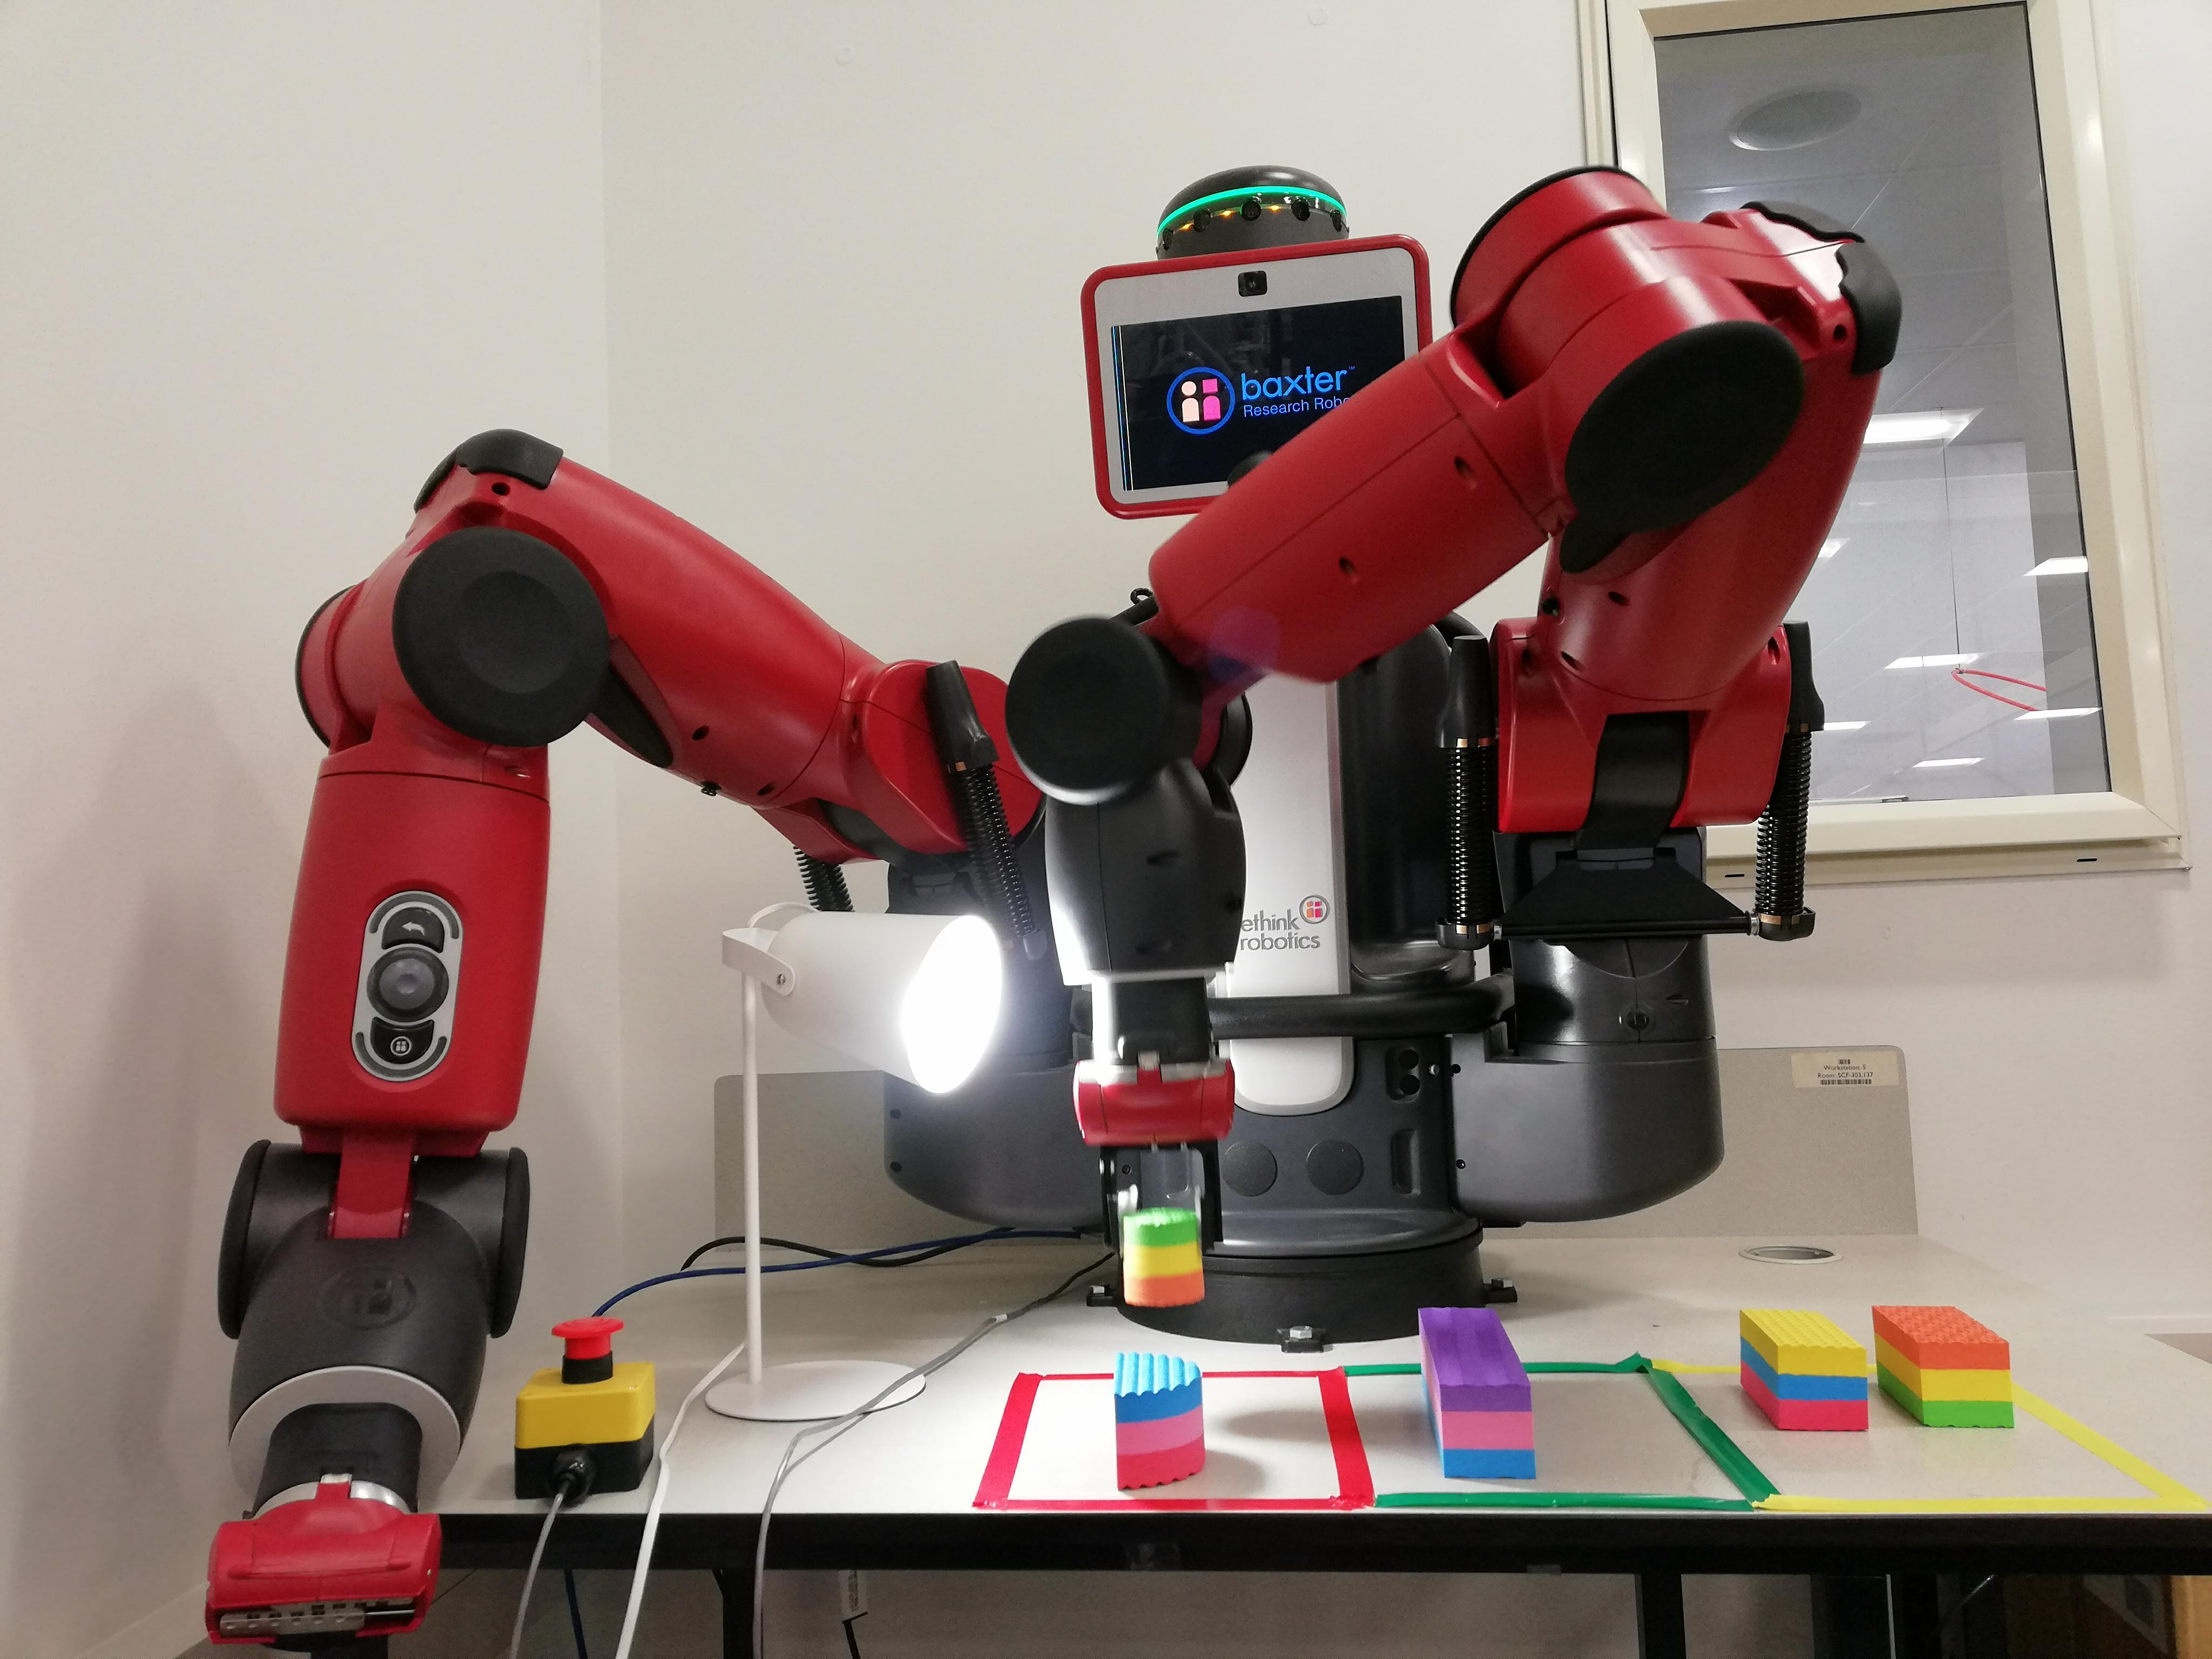
\includegraphics[width=\textwidth]{Images/baxter1}
      \caption{Baxter robot.}
      \label{fig:example-baxter}
    \end{subfigure}
    \begin{subfigure}{0.17\textwidth}
      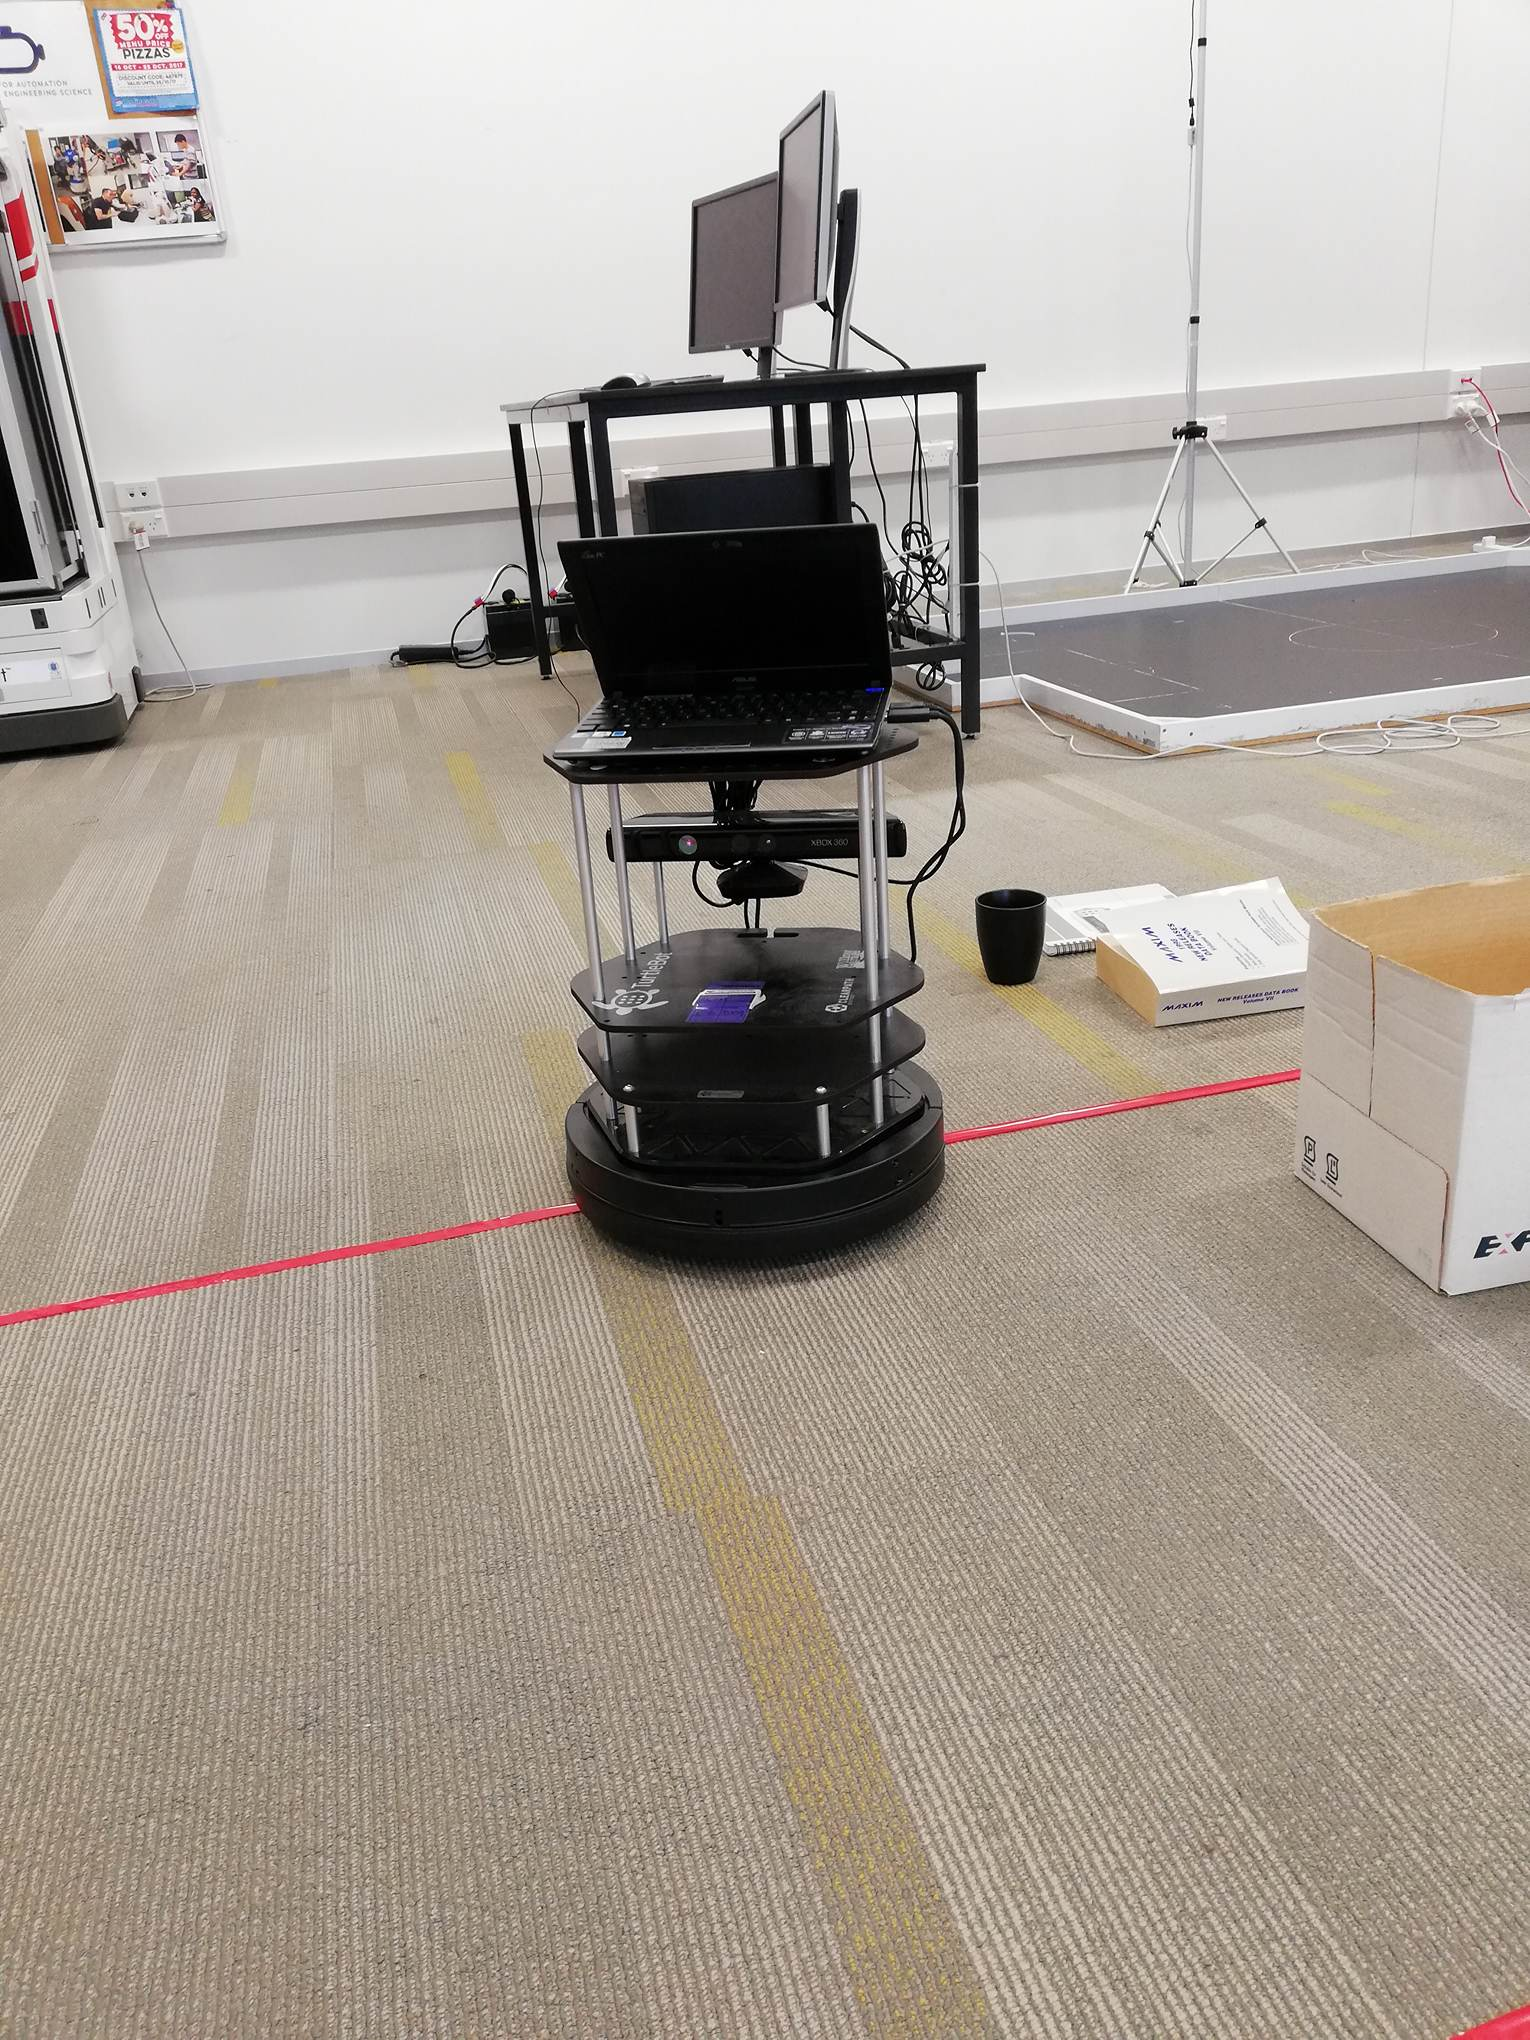
\includegraphics[width=\textwidth]{Images/turtlebot1}
      \caption{Turtlebot.}
      \label{fig:example-turtlebot}
    \end{subfigure}
  \end{center}
  \vspace{-1em}
  \caption{(a) Baxter robot manipulating objects on a tabletop; and
    (b) Turtlebot moving objects to particular locations in a lab.}
  \label{fig:example-robots}
  \vspace{-1em}
\end{figure}

% In this work we will focus on the implementation of a goal-oriented
% agent which is capable of reasoning with intentional actions in a
% changing complex environment. We put into practice a theory of
% commonsense reasoning with intentions, combined with a methodology for
% dealing with uncertainty and non-determinism at execution level while
% successfully reasoning at a higher abstract level with intention.



%%%%%%%%%%%%%%%%%%%%%%%%%%%%%%%%%%%%%%%%%%%%%%%%%%%%%%%%%%%%%%%%%%%%%%%%%%%%%%%%
%%%%%%%%%%%%%%%%%%%%%%%%%%%%%%%%%%%%%%%%%%%%%%%%%%%%%%%%%%%%%%%%%%%%%%%%%%%%%%%%
\section{Related Work}
\label{sec:relwork}
There is much work in the modeling and recognition of intentions,
e.g., belief-desire-intention (BDI) architectures for reasoning agents
model intention and guide reasoning by eliminating choices
inconsistent with current intentions~\cite{bratman1987intention}.
However, such architectures do not learn from past behavior, adapt to
new situations, or include an explicit representation of (or reasoning
about) goals.
 
An architecture formalizing intentions based on declarative
programming was presented in~\cite{baral2005reasoning}. It introduced
an action language that can represent intentions based on two
principles: (i) \emph{non-procrastination}, i.e., intended actions are
executed as soon as possible; and (ii) \emph{persistence}, i.e.,
unfulfilled intentions persist. This architecture was also used to
enable an external observer to recognize the activity of an observed
agent, i.e., for determining what has happened and what the agent
intends to do~\cite{gabaldon2009activity}. However, this architecture
did not support the modeling of agents that desire to achieve specific
goals. The more recent \emph{Theory of Intentions}
($\mathcal{TI}$)~\cite{blount2015theory,blount2014towards} builds
on~\cite{baral2005reasoning} to model the intentions of goal-driven
agents. This theory expanded transition diagrams with physical states
and physically executable actions to include mental fluents and
actions, associated a sequence of agent actions with the goal it
intended to achieve (called an ``activity''), and introduced an
\emph{intentional agent} that only performs actions that are intended
to achieve a desired goal and does so without delay.  This theory has
been used to create a methodology for understanding of narratives of
typical and exceptional restaurant
scenarios~\cite{zhang2017application}, and goal-driven agents in
dynamic domains have been modeled using such
activities~\cite{saribatur2017reactive}. A common requirement of such
theories and their use is that all the domain knowledge, including the
preconditions and effect of actions and potential goals, be known and
encoded in the knowledge base, which is difficult to do in robot
domains. Also, the set of states (and actions, observations) to be
considered can be large in robot domains, which makes efficient
reasoning challenging.  In~\cite{zhang2017application}, the authors
cluster indistinguishable states~\cite{zeynep2016logics} but these
clusters need to be encoded in advance. Furthermore, these approaches
do not consider the uncertainty in sensing and actuation.

Many logic-based approaches have been used in robotics, including
those that also support probabilistic
reasoning~\cite{hanheide:AIJ17,zhang:TRO15}. Algorithms based on
first-order logic do not support non-monotonic logical reasoning. ASP
addresses this limitation and has been used in cognitive robotics
applications~\cite{erdem2012applications,balduccini:iclp14}. The
classical ASP formulation does not support probabilistic models of
uncertainty, whereas many algorithms for sensing and actuation use
such models. Our prior refinement-based architecture reasoned with
tightly-coupled transition diagrams at two resolutions, executing each
abstract action in a coarse-resolution plan computed using ASP as a
sequence of concrete actions computed by probabilistic reasoning over
the relevant part of the fine-resolution
diagram~\cite{sridharan2017refinement,sridharan2016using}. This paper
explores the combination of ideas from $\mathcal{TI}$ and the
refinement-based architecture for robotics applications; these ideas
and differences from prior work are described below.


%%%%%%%%%%%%%%%%%%%%%%%%%%%%%%%%%%%%%%%%%%%%%%%%%%%%%%%%%%%%%%%%%%%%%%%%%%%%%%%%
%%%%%%%%%%%%%%%%%%%%%%%%%%%%%%%%%%%%%%%%%%%%%%%%%%%%%%%%%%%%%%%%%%%%%%%%%%%%%%%%
\section{Cognitive Architecture}
\label{sec:arch}

\begin{figure*}[tb]
\centering
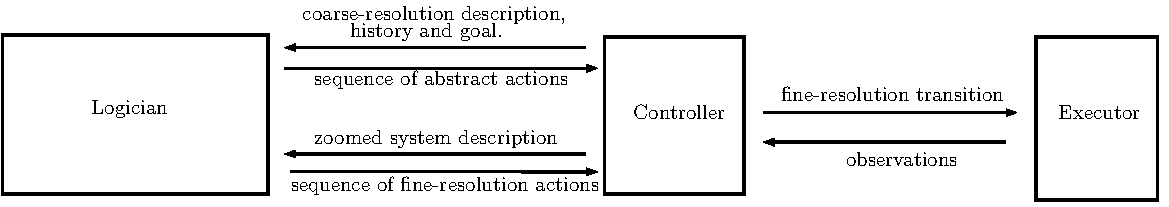
\includegraphics[width=0.95\textwidth]{Images/architecture.pdf}
\caption{Architecture uses logic representation of the world at two
  levels of resolution}
\label{fig:arch-overview}
\end{figure*}

Figure~\ref{fig:arch-overview} presents a block diagram of the overall
architecture. Similar to prior work~\cite{sridharan2017refinement},
this architecture may be viewed as consisting of three components:
controller, logician and executor. The controller is responsible for
holding the overall beliefs of domain state, and for the transfer of
control and information between all components. For any given goal,
the logician performs non-monotonic logical reasoning with the
coarse-resolution representation of commonsense knowledge to generate
an activity, i.e., a sequence of intentional abstract actions. Each
abstract action is implemented as a sequence of concrete actions;
these actions are executed probabilistically by the executor, with the
outcomes (and relevant observations) being communicated to the
controller and added to the coarse-resolution history of the logician.
These components are described below, along with differences from
prior work, using variants of the following illustrative domain.

\begin{example2}\label{ex:illus-example}[Robot Assistant (RA) Domain]
  {\rm Consider a robot assisting humans in moving particular objects
    to specific locations in an indoor office domain with:
    \begin{itemize}
    \item Sorts such as $place$, $thing$, $robot$, $object$, and
      $book$, arranged hierarchically, e.g., $object$ and $robot$ are
      subsorts of $thing$. Sort names and constants are in lower-case,
      and variable names are in uppercase.
    \item Places: $\{office_1, office_2, kitchen, library\}$ with a
      door between neighboring places; only door between $kitchen$ and
      $library$ can be locked---Figure~\ref{fig:places}.
    \item Instances of sorts, e.g., $rob_1$, $book_1$, $book_2$.
    \item Static attributes such as $color$, $size$ and different
      parts (e.g., $base$ and $handle$) associated with objects.
    \item Other agents that may influence the domain, e.g., move a
      book or lock a door. These agents are not modeled.
    \end{itemize}
  }
\end{example2}

\begin{figure}[tbh]
  \centering
  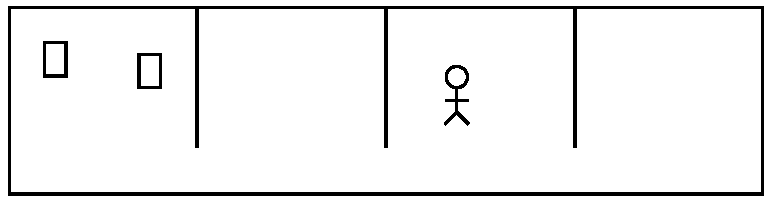
\includegraphics[width=0.95\columnwidth]{Images/fourrooms.pdf}
  \caption{Representation of four rooms in Example~\ref{fig:places},
    with a unknown human in the $kitchen$ and two books in $office_1$.
    Only door to library can be locked.}
  \label{fig:places}
\end{figure}

% The robot can $pick\_up$ and $put\_down$ books, $move$ from one room
% to another, or $unlock$ the $library$ door. In this domain, we also
% include two exogenous actions. One is an action of locking the door of
% the library, which we call $exo\_lock$ and another is moving a book to
% a different room, which we call $exo\_move$. These two actions are
% performed by one or more external agents that will not be represented
% in the domain. All there is in the domain is the representation of the
% exogenous actions. The objective of the robot, or his goal, would to
% put both books in the $library$.


%%%%%%%%%%%%%%%%%%%%%%%%%%%%%%%%%%%%%%%%%%%%%%%%%%%%%%%%%%%%%%%%%%%%%%%%%%%%%%%%
\subsection{Action Language and Domain Representation}
\label{sec:arch-ald}
Action languages are formal models of parts of natural language used
for describing the transition diagram of dynamic systems. We use
action language $\mathcal{AL}_d$~\cite{gelfond:ANCL13}, which has a
sorted signature with \emph{actions}, \emph{statics}, i.e., domain
attributes whose values cannot be changed by actions, and
\emph{fluents}, i.e., domain attributes whose values can be changed by
actions. Fluents can be \emph{inertial} (and obey laws of inertia) or
\emph{defined}.  A domain attribute \emph{p} or its negation is a
domain \emph{literal}.  $\mathcal{AL}_d$ allows three types of
statements: \emph{causal law}, \emph{state constraint}, and
\emph{executability condition}; some examples below.

The domain representation consists of system description
$\mathcal{D}$, a collection of statements of $\mathcal{AL}_d$, and
history $\mathcal{H}$. $\mathcal{D}$ has a sorted signature $\Sigma$
and axioms that describe the transition diagram $\tau$. $\Sigma$
defines the basic sorts, domain attributes and actions. Basic sorts of
the RA domain and some ground instances were introduced in
Example~\ref{ex:illus-example}. Domain attributes and actions are
described in terms of their arguments' sorts. Statics of the RA domain
include relations such as $next\_to(place, place)$. Fluents include
$loc(thing, place)$, the location of robot or objects---other agents'
locations are not modeled; $in\_hand(robot, object)$, which denotes a
particular object is in the robot's hand; and $locked(place)$, which
implies a particular place is locked.  Object attributes such as
$color$ and $size$ are assumed to be static.  Robot's actions include
$move(robot, place)$, $pickup(robot, object)$, $putdown(robot,
object)$, and $unlock(robot, place)$; we also consider exogenous
actions $exo\_move(object, place)$ and $exo\_lock(place)$ for
diagnostic reasoning. Relation $holds(fluent, step)$ implies a
particular fluent is true at a timestep.

Axioms for the RA domain include causal laws, constraints and
executability conditions such as:
\begin{align*}
  &move(rob_1, P)~~\mathbf{causes}~~loc(rob_1, P) \\
  &pickup(rob_1, O)~~\mathbf{causes}~~in\_hand(rob_1, O) \\
%  &\neg loc(E, L_2)~~\mathbf{if}~~loc(E, L_1),~ L_1\neq L_2 \\
  &loc(O, P)~~\mathbf{if}~~ loc(rob_1, P),~in\_hand(rob_1, O)\\
  &\mathbf{impossible}~~pickup(rob_1, O)~~\mathbf{if}~~loc(rob_1,
  L_1), loc(O, L_2)
\end{align*}
The history $\mathcal{H}$ of a dynamic domain is usually a record of
fluents observed to be true or false at a timestep, and the occurrence
of an action at a time step. We expand this notion to allow the
representation of defaults describing the values of fluents in their
initial states and exceptions (if any).

The domain representation is translated into a program
$\Pi(\mathcal{D}, \mathcal{H})$ in CR-Prolog\footnote{We use the terms
  ``ASP'' and ``CR-Prolog'' interchangeably.}, a variant of ASP that
incorporates consistency restoring (CR)
rules~\cite{balduccini:aaaisymp03}. ASP is based on stable model
semantics, and supports \emph{default negation} and \emph{epistemic
  disjunction}, e.g., unlike ``$\lnot a$'' that states \emph{a is
  believed to be false}, ``$not~a$'' only implies \emph{a is not
  believed to be true}.  ASP can represent recursive definitions and
constructs that are difficult to express in classical logic
formalisms. $\Pi$ includes the signature and axioms of $\mathcal{D}$,
inertia axioms, reality checks, and observations, actions, and
defaults from $\mathcal{H}$. Every default has a CR rule that allows
the robot to assume the default's conclusion is false to restore
consistency.  Algorithms for computing entailment, and for planning
and diagnostics, reduce these tasks to computing \emph{answer sets} of
CR-Prolog programs. We compute answer sets using the language
SPARC~\cite{balai:lpnmr13}.

%%%%%%%%%%%%%%%%%%%%%%%%%%%%%%%%%%%%%%%%%%%%%%%%%%%%%%%%%%%%%%%%%%%%%%%%%%%%%%%%
\subsection{Adapted Theory of Intention}
\label{sec:arch-toi}
For a given goal, a robot using ASP-based reasoning will compute a
plan and execute it until the goal is achieved or an action has an
unexpected outcome; in the latter case, the robot will try to explain
the outcome and compute a new plan. To motivate a need for a different
approach in dynamic domains, consider the following scenarios in which
the goal is to move $book_1$ and $book_2$ to the $library$; these have
been adapted from scenarios considered in prior
work~\cite{blount2015theory}:
\begin{itemize}
\item \textbf{Scenario 1 (planning):} Robot $rob_1$ is in the kitchen
  holding $book_1$, and believes $book_2$ is in the kitchen and
  library is unlocked. The computed plan is: $move(rob_1, library)$,
  $put\_down(rob_1, book_1)$, $move(rob_1, kitchen)$, $pickup(rob_1,
  book_2)$, $move(rob_1, library)$, $put\_down(rob_1, book_2)$.

\item \textbf{Scenario 2 (unexpected success):} Assume that $rob_1$ in
  Scenario-1 has moved to the $library$ and put $book_1$ down, and
  observes $book_2$ there. The robot should be able to explain this
  observation (e.g., $book_2$ was moved there) and realize the goal
  has been achieved.

\item \textbf{Scenario 3 (not expected to achieve goal, diagnose and
    replan, case 1):} Assume $rob1$ in Scenario-1 starts moving
  $book_1$ to $library$, but observes $book_2$ is not in the
  $kitchen$.  Now, $rob_1$ should realize the plan will fail, explain
  the observation and compute a new plan.

\item \textbf{Scenario 4 (not expected to achieve goal, diagnose and
    replan, case 2):} Assume $rob1$ is in the kitchen holding $book1$,
  and believes $book2$ is in $office_2$ and $library$ is unlocked. The
  robot plans to first put $book_1$ in the $library$ before fetching
  $book_2$ from $office_2$. Before $rob_1$ moves to the $library$, it
  suddenly observes $book_2$ in the $kitchen$.  Now, $rob_1$ should
  realize the plan will fail, explain the observation and compute a
  new plan.

\item \textbf{Scenario 5 (failure to achieve the goal, diagnose and
    replan):} Assume $rob_1$ in Scenario-1 is putting $book_2$ in the
  $library$, after having put $book_1$ in the $library$ earlier, and
  observes that $book_1$ is no longer there. The robot's intention
  should persist; it should explain the observation(s), replan if
  necessary, and execute actions until the goal is achieved.

% \item \textbf{Scenario 6: Failure to execute, diagnosis and
%     replanning:} Assume $rob_1$ in scenario 1 is unexpectedly unable
%   to execute the first action \stt{move($rob_1$, library)}. In this
%   case, $rob_1$ should reason that the door must be locked and create
%   a new plan whose first action is to unlock the $library$.
\end{itemize}
% Mohan, regarding the ToI mental fluents, there are both types,
% defined: active(#activity), in_progress(#activity),
% in_progress_goal(#possible_goal), next_action(#activity, #action).
% and inertial: active_goal(#possible_goal), status(#activity,
% #index_status), next_name(#activity_name).
%% 
% None of these are directly changed by an external physical action. The
% only fluent that is related to the physical world, in a way is
% "status", which will change if: 1 an intended agent action has taken
% place and the status of the activity has therefore changed or 2. if
% the world has changed in a way that the activity will not be
% successful any longer and the status of the activity becomes -1.
To support the desired behavior in such scenarios, we build on the
principles of non-procrastination and persistence and the ideas from
$\mathcal{TI}$. Our architecture enables the robot to compute actions
that are intended given any goal and its current beliefs. As the robot
attempts to implement each such action, \emph{it obtains all
  observations relevant to this action and the intended goal}, and
adds these observations to history. We denote this adapted theory of
intention component as $\mathcal{ATI}$. This component first extends
$\Sigma$ to represent an \emph{activity}, a triplet of a \emph{goal},
a \emph{plan} to achieve the goal, and a \emph{name}, by introducing
relations such as:
\begin{align*}
  &activity(name),~~activity\_goal(name, goal)\\
  &activity\_length(name, length)\\
  &activity\_component(name, number, action)
\end{align*}
for named activities, and the actions, length and goal corresponding
to an activity---when ground, these relations are statics. The
existing fluents of $\Sigma$ are considered \emph{physical fluents}
and are expanded to include \emph{mental fluents}, e.g.:
\begin{align*}
  &active\_activity(activity),~next\_action(activity, action)\\
  &in\_progress\_activity(activity),~in\_progress\_goal(goal)\\
  &active\_goal(goal),~next\_activity\_name(name)\\
  &current\_action\_index(activity, index)
\end{align*}
where relations in the top two lines are defined fluents, whereas the
others are inertial fluents. These fluents represent the robot's
belief about a specific action, activity, or goal being active or in
progress. None of these are changed directly by a physical action; the
\emph{current\_action\_index} can change if the robot has completed an
intended action or if a change in the domain makes it impossible for
an activity to succeed. Next, existing actions in $\Sigma$ are
considered \emph{physical actions}, and expanded to include
\emph{mental actions} such as:
\begin{align*}
  &start(name),~~stop(name),~~select(goal)\\
  &abandon(goal)
\end{align*}
where the first two are used by the controller to start or stop an
activity, and the other two are exogenous actions exercised (say, by a
human) to select or abandon a goal.

We also define new axioms in $\mathcal{AL}_d$, e.g., to represent the
effects of actions, prevent certain outcomes, and generate intentional
actions---we do not describe these here due to space constraints. The
notion of history is also expanded to include: $attempt(action,
step)$, which denotes an action was attempted at a time step, and
$\neg~hpd(action, step)$, which denotes an action did not happen at a
time step. The revised system description and history are translated
automatically to CR-Prolog program $\Pi(\mathcal{D}', \mathcal{H}')$
that is solved for planning or diagnostics. The program for the RA
domain is available online~\cite{code-results}.

%\footnote{\url{https://github.com/hril230/theoryofintentions/tree/master/simmulation}}.

% The new control strategy is an extension of the $\mathcal{AIA}$
% presented in \cite{blount2015theory}, with the addition of the steps
% relevant to zooming at fine-resolution. The control strategy starts
% after given a desired goal, and it starts with observing the world.
% Then the control loop does as follows:
% \begin{enumerate}
% \item interpret observations,
% \item \emph{logician} find next intended action, 
% \item zoom in to fine-resolution ASP to create a sequence of
%   fine-resolution,
% \item fore each fine-resolution action:
%   \begin{itemize}
%   \item attempts to execute the next action, 		
%   \item observes the effect of his attempt. 
%   \end{itemize}
% \item update history with a record of the attempt of the
%   coarse-resolution,
% \item observe the world, update history with observations, go to
%   step1.
% \end{enumerate}
% One of the main differences between the two architectures is that an
% agent with the Theory of Intentions would observe all objects defined
% in his domain relevant to the goal during the execution process, as
% well as all outcomes relevant to the action he is executing at the
% time, and reason about these observations in regards to his intention.
% A traditional agent would only observe and reason about objects and
% states that are relevant to the action he is executing. The time used
% for reasoning about these observations is a disadvantage for the
% intentional agent, but it may be trade off when his reasoning helps to
% achieve this goal, or do it in a more efficient manner. We will
% investigate this trade off later.

Key differences between $\mathcal{ATI}$ and $\mathcal{TI}$ are:
\begin{itemize}
\item $\mathcal{TI}$ becomes computationally expensive, especially as
  the size of the plan or history increases. It also performs
  diagnostics and planning jointly, which allows it to consider
  different explanations during planning but increases computational
  cost in complex domains. $\mathcal{ATI}$, on the other hand, first
  builds a consistent model of history by considering different
  explanations, and \emph{uses this model to guide planning},
  significantly reducing computational cost in complex domains.
\item Unlike $\mathcal{TI}$, we make the realistic assumption that the
  robot does not have access to the state of the agents (e.g., humans)
  that may perform exogenous actions; any exogenous actions can only
  be inferred.
\item $\mathcal{ATI}$ does not include the notion of sub-goals and
  sub-activities (and associated relations) from $\mathcal{TI}$, as
  they were not necessary; these may be introduced later without loss
  of generality of our overall architecture.
% \item In our architecture, the robot only acts upon a previously
%   selected goal, and it will finish any action or intention once the
%   goal has been reached. It does not include the action $wait$, which
%   is used in the original model as the agent's intended action while
%   no specific goal has been selected.
% \item The original system was developed in CR-Prolog in which a
%   preference over two different consistency rules can be specified.
%   We have developed our ASP program in Spark, and that preference can
%   not be specified. This has made it not possible for our system to
%   explicitly tell by the logician when a goal is futile. Our ASP will
%   simple consider the description of the domain with a futile goal as
%   inconsistent.
\end{itemize}
Any architecture using $\mathcal{TI}$, and others based on
logic-programming or classical first-order logic, often have two key
limitations. First, the coarse-resolution representation discussed so
far (e..g, places and objects) is not sufficient for most tasks to be
performed by the robot, e.g., to move to a particular location or
grasp a particular object, and reasoning logically over a more
fine-grained domain representation will be computationally intractable
for complex domains. Second, we have not yet modeled the actual
sensor-level observations of the robot or the uncertainty in sensing
and actuation. Section~\ref{sec:relwork} discusses the limitations of
other approaches based on logical and/or probabilistic reasoning. Our
architecture seeks to address these limitations by combining
$\mathcal{ATI}$ with ideas drawn from work on a refinement-based
architecture~\cite{sridharan2017refinement}.


%%%%%%%%%%%%%%%%%%%%%%%%%%%%%%%%%%%%%%%%%%%%%%%%%%%%%%%%%%%%%%%%%%%%%%%%%%%%%%%%
\subsection{Refinement, Zooming and Execution}
\label{sec:arch-refine-zoom}
Consider a coarse-resolution system description $\mathcal{D}_c$ of
transition diagram $\tau_c$ that includes the $\mathcal{ATI}$. For any
given goal, reasoning with $\Pi(\mathcal{D}_c, \mathcal{H}_c)$, as
described above, will provide an activity, i.e., a sequence of
abstract intentional actions. The execution of the coarse-resolution
transition corresponding to each such action is based on a
fine-resolution system description $\mathcal{D}_f$ of transition
diagram $\tau_f$, which is a \emph{refinement} of, and tightly coupled
to, $\mathcal{D}_c$. We can imagine refinement as taking a closer look
at the domain through a magnifying lens, potentially leading to the
discovery of structures that were previously abstracted away by the
designer~\cite{sridharan2017refinement}. $\mathcal{D}_f$ is
constructed automatically as a step in the design methodology using
$\mathcal{D}_c$ and some domain-specific information that has to be
provided by the designer.

The signature $\Sigma_f$ of $\mathcal{D}_f$ includes each basic sort
of $\mathcal{D}_c$ whose elements have not been \emph{magnified} by
the increase in resolution, or both the coarse-resolution copy and its
fine-resolution \emph{counterparts} for sorts with magnified elements.
In the RA domain, this would include the original set of places,
$places^*$, and $place=\{c_1,\dots,c_m\}$, i.e., cells in those
places; cups may, in a similar manner, have a $base$ and $handle$.  We
also include domain-dependent statics relating the magnified objects
and their counterparts, e.g., $component(cup\_base, cup)$.  Next,
domain attributes of $\Sigma_f$ include the coarse-resolution version
and fine-resolution counterparts (if any) if each domain attribute of
$\Sigma_c$. For instance, $\Sigma_f$ will include both
$next\_to(place, place)$ and $next\_to^*(place^*, place^*)$---the
former describes two cells that are next to each other while the
latter describes two rooms that are next to each other. Actions of
$\Sigma_f$ include (a) every action in $\Sigma_c$ with its magnified
parameters replaced by fine-resolution counterparts; and (b)
knowledge-producing action $test(robot, fluent)$ that checks the value
of a fluent in a given state.  Finally, $\Sigma_f$ includes
\emph{knowledge fluents} to describe observations of the environment
and the axioms governing them, e.g., inertial fluents to describe the
direct (sensor-based) observation of the values of the fine-resolution
fluents, and defined domain-dependent fluents that determine when the
value of a particular fluent can be tested. The $test$ actions only
change the values of knowledge fluents.

The axioms of $\mathcal{D}_f$ include (a) axioms of $\mathcal{D}_c$
with variables ranging over appropriate sorts from $\Sigma_f$; (b)
axioms for observing the domain through sensor inputs; and (c) axioms
relating coarse-resolution domain attributes with their
fine-resolution counterparts. For example:
\begin{align*}
  &test(rob_1, F) ~{\bf causes}~~dir\_obs(rob_1,F)~~{\bf if }~~F=true \\
  &{\bf impossible}~~test(rob_1, F)~~{\bf if}~~\lnot can\_test(rob_1, F) \\
  &in\_hand^*(rob_1, O) ~{\bf if}~~component(O\_base, O),\\
  &~~~~~~~~~~~~~~~~~~~~~~~~~~~~~~in\_hand(rob_1, O\_base)
\end{align*} 
If certain conditions are met, e.g., each coarse-resolution domain
attribute can be defined in terms of the fine-resolution attributes of
the corresponding components, there is a path in $\tau_f$ for each
transition in $\tau_c$---see~\cite{sridharan2017refinement} for
details.

Reasoning at fine resolution using $\mathcal{D}_f$ does not address
the uncertainty in sensing and actuation, and becomes computationally
intractable for complex domains. We address this problem by drawing on
the principle of \emph{zooming} introduced
in~\cite{sridharan2017refinement}.  Specifically, for each abstract
transition $T$ to be implemented (i.e., executed) at fine resolution,
we automatically determine the system description $\mathcal{D}_f(T)$
relevant to this transition; we do so by determining the relevant
object constants and restricting $\mathcal{D}_f$ to these object
constants. To implement $T$, we then use ASP-based reasoning with
$\Pi(\mathcal{D}_f(T), \mathcal{H}_f)$ to plan a sequence of
\emph{concrete} (i.e., fine-resolution) actions. In what follows, we
use ``refinement and zooming'' to refer to the use of both refinement
and zooming as described above. Note that fine-resolution reasoning
does not (need to) use $\mathcal{ATI}$.

The actual execution of the plan of concrete action is based on
existing implementations of probabilistic algorithms for common
robotics tasks such as motion planning, object recognition and
localization. The high-probability outcomes of each action's execution
are elevated to statements associated with complete certainty in
$\mathcal{H}_f$ and used for subsequent reasoning. The outcomes from
fine-resolution execution of each abstract transition, along with
relevant observations, are added to $\mathcal{H}_c$ for subsequent
reasoning using $\mathcal{ATI}$. The CR-Prolog programs for
fine-resolution reasoning and the program for the overall control loop
are available online~\cite{code-results}.

Key differences between the current representation and use of
fine-resolution information, and prior
work~\cite{sridharan2017refinement} are:
\begin{itemize}
\item Prior work used a partially observable Markov decision process
  (POMDP) to reason probabilistically over the zoomed fine-resolution
  system description $\mathcal{D}_f(T)$ for any coarse-resolution
  transition $T$; this can be computationally expensive, especially
  when domain changes prevent reuse of POMDP
  policies~\cite{sridharan2017refinement}. In this paper, CR-Prolog is
  used to compute a plan of concrete actions from $\mathcal{D}_f(T)$;
  each concrete action is executed using probabilistic algorithms that
  use the corresponding models of uncertainty, significantly reducing
  the computational costs of fine-resolution planning and execution.

\item Prior work did not (a) reason about intentional actions; (b)
  maintain any fine-resolution history; or (c) obtain and exploit all
  the information from fine-resolution observations. The architecture
  described in this paper keeps track of the relevant fine-resolution
  observations and adds appropriate statements to the
  coarse-resolution history to use all relevant information. It also
  explicitly builds a consistent model of history at fine-resolution.
\end{itemize}


%%%%%%%%%%%%%%%%%%%%%%%%%%%%%%%%%%%%%%%%%%%%%%%%%%%%%%%%%%%%%%%%%%%%%%%%%%%%%%%%
%%%%%%%%%%%%%%%%%%%%%%%%%%%%%%%%%%%%%%%%%%%%%%%%%%%%%%%%%%%%%%%%%%%%%%%%%%%%%%%%
\section{Experimental Setup and Results}
\label{sec:expres}
This section reports the results of experimentally evaluating the
capabilities of our architecture in different scenarios.  We evaluated
the following hypotheses:
\begin{itemize}
\item \underline{\textbf{H1:}} using $\mathcal{ATI}$ improves the
  computational efficiency in comparison with not using it, especially
  in scenarios with unexpected success.
\item \underline{\textbf{H2:}} using $\mathcal{ATI}$ improves the
  accuracy in comparison with not using this component, especially in
  scenarios with unexpected goal-relevant observations.
\item \underline{\textbf{H3:}} architecture that combines
  $\mathcal{ATI}$ with refinement and zooming supports reliable and
  efficient operation in complex robot domains.
\end{itemize}
To evaluate these hypotheses, we ran experimental trials: (a) in a
simulated domain based on Example~\ref{ex:illus-example}; (b) on a
Baxter robot manipulating objects on a tabletop; and (c) on a
Turtlebot finding and moving objects to specific locations in an
indoor domain. In each trial, the robot's goal was to find and move
one or more objects to particular locations. As a baseline for
comparison, we used an ASP-based reasoner that does not include
$\mathcal{ATI}$---we refer to this as the ``traditional planning''
($\mathcal{TP}$) approach in which only the outcome of the action
currently being executed is monitored. To evaluate the hypotheses, we
used one or more of the following performance measures: (i) total
planning and execution time; (ii) number of plans computed; (iii)
planning time; (iv) execution time; (v) number of actions executed;
and (vi) accuracy.

\begin{table*}[t]
\centering
\small
\setlength\arrayrulewidth{0.5pt}
\begin{tabular}{|c|c|c|c|c|c|c|c|}
 \hline
\multirow{2}{*}{Scenarios}&  \multicolumn{5}{|c|}{Average Ratios} & \multicolumn{2}{|c|}{Accuracy}\\
 \cline{2-8}
&Total Time &Number Plans &Planning Time &Exec. Time &Exec.Steps & $\mathcal{TP}$ & $\mathcal{ATI}$ \\
\hline
 1 &0.81 &1.00 &0.45  &1.00 &1.00 &100\% &100\% \\
 \hline
 2 &3.06 &2.63 &1.08 &5.10 &3.61 &100\% &100\% \\
 \hline
3 &0.81 &0.92 &0.34 &1.07 &1.12 &72\% &100\% \\
 \hline
4 &1.00 &1.09 &0.40 &1.32 &1.26 &73\% &100\% \\
 \hline
5 &0.18 &0.35 &0.09 &0.21 &0.28 &0\%   &100\% \\
 \hline
 All &1.00 & 1.08 &0.41 &1.39 &1.30 &74\% &100\% \\
 \hline
 3 - no failures &1.00 &1.11 &0.42 &1.32 &1.39 &100\% &100\% \\
 \hline
 4 - no failures  &1.22 &1.31 &0.49 &1.61 &1.53 &100\% &100\% \\
 \hline
 All - no failures &1.23&1.30 &0.5 &1.72 &1.60 &100\% &100\% \\
\hline
\end{tabular}
\caption[Results]{Experimental results comparing $\mathcal{ATI}$ with $\mathcal{TP}$ in different scenarios. Values of all performance measures (except accuracy) for $\mathcal{TP}$ are expressed as a fraction of the values of the same measures for $\mathcal{ATI}$. We notice that $\mathcal{ATI}$ improves accuracy and computational efficiency, especially in dynamic domains.}
\label{tab:sim-results}
\end{table*}

% One of the characteristics of an intentional agent is that, during the
% execution of the plan, the agent reasons about all the observed values
% of his domain that are relevant to the goal, as well as the
% observations relevant to the action he is executing at the time.
% However, a traditional agent would only reason about observations of
% objects and states that are relevant to the action he is executing.
% The time used for reasoning about these observations is a disadvantage
% for the intentional agent, but it may be trade off when his reasoning
% helps to achieve his goal, or do it in a more efficient manner. 

%%%%%%%%%%%%%%%%%%%%%%%%%%%%%%%%%%%%%%%%%%%%%%%%%%%%%%%%%%%%%%%%%%%%%%%%%%%%%%%%
\subsection{Experimental Results (Simulation)}
\label{sec:expres-sim}
We first evaluated hypotheses H1 and H2 extensively in a simulated
world that mimics Example~\ref{ex:illus-example}, with four places and
different objects. Please also note the following:
\begin{itemize}
\item To fully explore the effects of $\mathcal{ATI}$, we did not
  include refinement in these simulated trials, i.e., the robot only
  reasons with the coarse-resolution domain representation. We also
  temporarily abstracted away uncertainty in perception and actuation.

\item We conducted paired trials and compared the results obtained
  with $\mathcal{TP}$ and $\mathcal{ATI}$ for the same initial
  conditions and for the same dynamic domain changes (when
  appropriate), e.g., a book is moved unknown to the robot and the
  robot obtains an unexpected observation.

\item To measure execution time, we assumed a fixed execution time for
  each concrete action, e.g., $15$ units for moving from a room to the
  neighboring room, $5$ units to pick up an object or put it down; and
  $5$ units to open a door. Ground truth is provided by a component
  that reasons with complete domain knowledge.
\end{itemize}
Table~\ref{tab:sim-results} summarizes the results of $\approx 800$
paired trials in each scenario described in
Section~\ref{sec:arch-toi}; all claims made below were tested for
statistical significance. The initial conditions, e.g., starting
location of the robot and objects' locations, and the goal were set
randomly in each paired trial; the simulation ensures that the goal is
reachable from the chosen initial conditions. Also, in suitable
scenarios, a randomly-chosen, valid (unexpected) domain change is
introduced in each paired trial. Given the differences between paired
trials, it does not make sense to average the measured time or plan
length across different trials. In each paired trial, the value of
each performance measure (except accuracy) obtained with
$\mathcal{TP}$ is thus expressed as a fraction of the value of the
same performance measure obtained with $\mathcal{ATI}$; each value
reported in Table~\ref{tab:sim-results} is the average of these
computed ratios. We highlight some key results below.

% In each trial, for each time-step of the simulation run, an exogenous
% action was activated with probability 0.12. If the exogenous action
% was activated, one of two actions was chosen with the same
% probability: move book1 or move book2. Then a location (different from
% the current location of the book) will be chosen at random.  The
% exogenous action will happen only if the conditions are possible, for
% example a chosen $exo\_move(book1,kitchen)$ would not happen if the
% agent was holding $book1$, and $exo\_lock(library)$ would not happen
% if the library was locked. At most one exogenous action is triggered
% in each trial.
Scenario-1 represents a standard planning task with no unexpected
domain changes. Both $\mathcal{TP}$ and $\mathcal{ATI}$ provide the
same ($100\%$) accuracy and compute essentially the same plans, but
reasoning with intentions to compute plans takes longer. This explains
the reported average values of $0.45$ and $0.81$ for planning and
total time in Table~\ref{tab:sim-results}.

In Scenario-2 (unexpected success), both $\mathcal{TP}$ and
$\mathcal{ATI}$ achieve $100\%$ accuracy. Here, $\mathcal{ATI}$ stops
reasoning and execution once it realizes the desired goal has been
achieved unexpectedly. However, $\mathcal{TP}$ does not realize this
because it does not consider observations not directly related to the
action being executed; it keeps trying to find the objects of interest
in different places. This explains why $\mathcal{TP}$ has a higher
planning time and execution time, and also computes many more plans
and executes more plan steps than $\mathcal{ATI}$.

Scenarios 3--5 correspond to different kinds of unexpected failures.
In all trials corresponding to these scenarios, $\mathcal{ATI}$ leads
to successful achievement of the goal, but there are a significant
number of instances in which $\mathcal{TP}$ is unable to recover from
the unexpected observations and achieve the goal. For instance, if the
goal is to move two books to the library, and one of the books is
moved to an unexpected location when it is no longer part of an action
in the robot's plan, the robot may not reason about this unexpected
occurrence and will thus fail to achieve the goal. This phenomenon is
especially pronounced in Scenario-5 that represents an extreme case in
which the robot using $\mathcal{TP}$ is never able to achieve the
desired goal because it never realizes that it has failed to achieve
the goal. Notice that in the trials corresponding to all three
scenarios, $\mathcal{ATI}$ takes more time than $\mathcal{TP}$ to plan
and execute the plans, but this increase in time is justified by the
high accuracy and the desired behavior in these scenarios.

The row labeled ``All'' summarizes the results across the different
scenarios.  The following three rows summarize results after removing
all trials in which $\mathcal{TP}$ fails to achieve the assigned goal.
We then notice that $\mathcal{ATI}$ is at least as fast as
$\mathcal{TP}$ and is often faster, i.e., takes less time (overall) to
plan and execute actions to achieve the desired goal. In summary,
$\mathcal{TP}$ results in faster planning but results in lower
accuracy and higher execution time than $\mathcal{ATI}$ in dynamic
domains, especially in the presence of unexpected successes and
failures that are common in dynamic robot domains. All these results
provide evidence in support of hypotheses H1 and H2.


% \comment{When failure cases are removed from scenarios 3, 4, all; ATI
%   is at least as fast as traditional planning}.  \comment{Effects of
%   ATI+refinement are seen better when plan execution time
%   significantly outweighs planning time}.



%%%%%%%%%%%%%%%%%%%%%%%%%%%%%%%%%%%%%%%%%%%%%%%%%%%%%%%%%%%%%%%%%%%%%%%%%%%%%%%%
\subsection{Execution traces}
\label{sec:expres-traces}
The following execution traces exemplify the differences in decision
making between the robot using  intentional agent and a traditional planning
agent when an exogenous action happens in the domain.

\begin{execexample}\label{exec:example1}[Example of Scenario-2]\\
  {\rm Assume that robot $rob_1$ is in the $kitchen$ initially,
    holding $book_1$ in its hand, and believes that $book_2$ is in
    $office_2$ and the $library$ is unlocked.
    \begin{itemize}
    \item The goal is to have $book_1$ and $book_2$ in the $library$.
      The computed plan is the same for $\mathcal{ATI}$ and
      $\mathcal{TP}$, and consists of actions:
      \begin{align*}
        &move(rob_1, library),~put\_down(rob_1, book_1),\\
        &move(rob_1, kitchen), ~move(rob_1, office_2),\\
        &pickup(rob_1, book_2), ~move(rob_1, kitchen)\\
        &move(rob_1, library), ~putdown(rob_1, book_2)
      \end{align*}
      
    \item Assume that as the robot is putting $book_1$ down in the
      $library$, someone has moved $book_2$ to the $library$.

    \item With $\mathcal{ATI}$, the robot observes $book_2$ in the
      $library$, reasons and explains the observation as the result of
      an exogenous action, realizes the goal has been achieved and
      stops further planning and execution.

    \item With $\mathcal{TP}$, the robot does not observe or does not
      use the information in the observation of $book_2$. It will thus
      waste time executing subsequent steps of the plan until it is
      unable to find or pickup $book_2$ in the $library$. It will then
      replan (potentially including prior observation of $book_2$) and
      eventually achieve the desired goal. It may also compute and
      pursue plans assuming $book_2$ is in different places, and take
      more time to achieve the goal.
    \end{itemize}
  }
\end{execexample}

\begin{execexample}\label{exec:example2}[Example of Scenario-5]\\
  {\rm Assume that robot $rob_1$ is in the $kitchen$ initially,
    holding $book_1$ in its hand, and believes that $book_2$ is in
    $kitchen$ and the $library$ is unlocked.
    \begin{itemize}
    \item The goal is to have $book_1$ and $book_2$ in the $library$.
      The computed plan is the same for $\mathcal{ATI}$ and
      $\mathcal{TP}$, and consists of the actions:
      \begin{align*}
        &move(rob_1, library),~put\_down(rob_1, book_1),\\
        &move(rob_1, kitchen), pickup(rob_1, book_2),\\
        &move(rob_1, library), ~putdown(rob_1, book_2)
      \end{align*}
    
    \item Assume the robot is in the act of putting $book_2$ in the
      $library$, after having already put down $book_1$ in the
      $library$ earlier. However, someone has moved $book_1$ to
      the $kitchen$ while the robot was moving $book_2$.

    \item With $\mathcal{ATI}$, the robot observes $book_1$ in not in
      the $library$, realizes the goal has not been achieved, and
      continues to replan until it finds $book_1$ and moves it to the
      $library$.

    \item With $\mathcal{TP}$, the robot puts $book_2$ in the
      $library$ and stops execution because it believes it has
      achieved the desired goal. In other words, it does not even
      realize that the goal has not been achieved.
    \end{itemize}
  }
\end{execexample}


%%%%%%%%%%%%%%%%%%%%%%%%%%%%%%%%%%%%%%%%%%%%%%%%%%%%%%%%%%%%%%%%%%%%%%%%%%%%%%%%
\subsection{Robot Experiments}
\label{sec:expres-robots}
We also ran experimental trials with the combined architecture, i.e.,
$\mathcal{ATI}$ with refinement and zoom, on two different robot
platforms. These trials represented instances of the different
scenarios (in Section~\ref{sec:arch-toi}) in domains that are variants
of the domain in Example~\ref{ex:illus-example}.

First, consider the experiments with the Baxter robot manipulating
objects on a tabletop as shown in Figure~\ref{fig:example-baxter}.
Some other details of the domain include:
\begin{itemize}
\item The goal is to move particular objects between different
  ``zones'' (instead of places) or specific (cell) locations on a
  tabletop.
\item After refinement, each zone is magnified to obtain grid cells.
  Also, each object is magnified into parts such as $base$ and
  $handle$ after refinement.
\item Objects are characterized by $color$ and $size$.
\item The robot cannot move but it can use its arm to move objects
  between cells or zones.
\end{itemize}

Next, consider the experiments with the Turtlebot robot operating in
an indoor domain as shown in Figure~\ref{fig:example-turtlebot}. Some
other details of the domain include:
\begin{itemize}
\item The goal is to find and move particular objects between places
  in an indoor domain.
\item The robot does not have a manipulator arm; it solicits help from
  a human to pickup the desired object when it has reached the desired
  source location and found the object, and to put the object down
  when it has reached the desired target location.
\item Objects are characterized by $color$ and $type$.
\item After refinement, each place/region was magnified to obtain grid
  cells. Also, each object is magnified into parts such as $base$ and
  $handle$ after refinement.
\end{itemize}
Although the two domains differ significantly, e.g., in the domain
attributes, actions and complexity, no change is required in the
architecture or the underlying methodology. Other than providing the
domain-specific information, no human supervision is necessary; most
of the other steps can be automated. In $\approx 50$ experimental
trials in each domain,the robot using the combined architecture is
able to successfully achieve the assigned goal. The performance is
similar to that observed in the simulation trials. For instance, if we
do not include $\mathcal{ATI}$, the robot has lower accuracy or takes
more time to achieve the goal in the presence of unexpected success or
failure; in other scenarios, the performance with $\mathcal{ATI}$ and
$\mathcal{TP}$ is comparable. Also, if we do not include zooming, the
robot takes a significantly longer to plan and execute concrete, i.e.,
fine-resolution actions. In fact, as the domain becomes more complex,
i.e., there are many objects and achieving the desired goal requires
plans with several steps, there are instances when the planning starts
becoming computationally intractable. All these results provide
evidence in support of hypothesis H3.

Videos of the trials on the Baxter robot and Turtlebot corresponding
to different scenarios can be viewed
online\footnote{\url{https://drive.google.com/drive/u/1/folders/1cWXVib82K7qVSIP5i_cT7HEBfE5cGB4G}}.
For instance, in one trial involving the Turtlebot, the goal is to
have both a cup and a bottle in the $library$, and these objects and
the robot are initially in $office_2$. The computes plan is for the
robot to pick up the bottle, move to the $kitchen$, move to the
$library$, put the bottle down, move back to the $kitchen$ and then to
$office_2$, pick up the cup, move to the $library$ through the
$kitchen$, and put the cup down. When the Turtlebot is moving to the
$library$ holding the bottle, someone moves the cup to the $library$.
With $\mathcal{ATI}$, the robot uses the observation of the cup, once
it has put the bottle in the $library$, to infer the goal has been
achieved and thus stops planning and execution. With just
$\mathcal{TP}$, the robot continued with its initial plan and realized
there was a problem only when it went back to $office_2$ and did not
find the cup.

Similarly, in one trial with the Baxter, the goal is to have blue and
green blocks in zone Y (right side of the screen) and these blocks are
initially in zone R (left side of the screen). The computed plan has
the Baxter move its arm to zone R, pick up a block, move to zone G
(center) then to zone Y to put the block down, and repeat this process
until it has moved all blocks. When the Baxter has moved one block and
is moving back to pick up the second block from zone R, an exogenous
action puts the first block in zone G (center). With $\mathcal{ATI}$,
as the Baxter is moving over zone G on the way to zone R, it observes
the block (it had previously put in zone Y), performs diagnostics and
realizes his current activity will not achieve the goal. It then
re-plans and manages to move all blocks to zone Y. With
$\mathcal{TP}$, the robot is not able to use the observation of the
first block in zone G, continues with the initial plan and never
realizes that the goal has not been achieved.



%%%%%%%%%%%%%%%%%%%%%%%%%%%%%%%%%%%%%%%%%%%%%%%%%%%%%%%%%%%%%%%%%%%%%%%%%%%%%%%%
\section{Discussion and Future Work}
In this paper we presented a generic architecture that reasons with
transition diagrams at two resolutions. Non-monotonic logical
reasoning with a coarse-resolution domain representation containing
commonsense knowledge is used to provide a plan of abstract
intentional actions for any given goal.  Each such abstract action is
implemented as a sequence of concrete actions by reasoning with the
relevant part of a fine-resolution representation that is a refinement
of the coarse-resolution representation. This architecture improves
the accuracy and computational efficiency of decision making in
different complex domains. In the future, we will explore and formally
establish the relationship between the different transition diagrams
in this architecture, along the lines of the analysis provided
in~\cite{sridharan2017refinement}. This will enable us to prove
correctness and provide other guarantees about the robot's
performance. We will also instantiate the architecture in different
domains and to further demonstrate the applicability of the
architecture. The long-term goal will be enable robots to represent
and reason reliably and efficiently with different descriptions of
knowledge and uncertainty.

%%%%%%%%%%%%%%%%%%%%%%%%%%%%%%%%%%%%%%%%%%%%%%%%%%%%%%%%%%%%%%%%%%%%%%%%%%%%%%%%
\section*{Acknowledgments}
The authors thank Michael Gelfond for discussions related to the
$\mathcal{TI}$ architecture~\cite{blount2015theory} and his
contributions to the refinement-based
architecture~\cite{sridharan2017refinement} we build on in this paper.
The authors also thank Evgenii Balai for providing support with the
SPARC software.


%%%%%%%%%%%%%%%%%%%%%%%%%%%%%%%%%%%%%%%%%%%%%%%%%%%%%%%%%%%%%%%%%%%%%%%%%%%%%%%%

\bibliographystyle{aaai} 
\bibliography{bibliography}

%%%%%%%%%%%%%%%%%%%%%%%%%%%%%%%%%%%%%%%%%%%%%%%%%%%%%%%%%%%%%%%%%%%%%%%%%%%%%%%%




\end{document}
